%-%-%-%-%-%-%-%-%-%-%-%-%-%-%-%-%-%-%-%-%-%-%-%-%-%-%-%-%-%-%-%-%-%-%-%-%-%-%
%%% MAIN DOCUMENT %%%

%-%-%-%-%-%-%-%-%-%-%-%-%-%-%-%-%-%-%-%-%-%-%-%-%-%-%-%-%-%-%-%-%-%-%-%-%-%-%

\documentclass[12pt, oneside]{book}
\usepackage{xcolor}
\usepackage{minted}

% \usepackage[T1]{fontenc}

\usepackage{draculatheme}
\newcommand{\documentTheme}{draculafg}
\newcommand{\documentLogo}{images/ML_logo_v2.png}
\newcommand{\documentBigLogo}{images/ML_logo_v2.png}
% \usemintedstyle{dracula}

% \newcommand{\documentBigLogo}{images/Hendrix Logo.png}
% \newcommand{\documentLogo}{images/small logo.png}
% \newcommand{\documentTheme}{black}

%%% AESTHETICS %%%
%-%-%-%-%-%-%-%-%-%-%-%-%-%-%-%-%-%-%-%-%-%-%-%-%-%-%-%-%-%-%-%-%-%-%-%-%-%-%


%%% Dimensions and Spacing %%%
\usepackage[margin=1in]{geometry}
\setlength{\parindent}{0pt}
\usepackage{setspace}
\usepackage{mathtools}
\linespread{1}
\usepackage{listings}
\usepackage{tikz}
\usetikzlibrary{shapes,backgrounds,calc,patterns,positioning}
\usepgflibrary{shadings}
\usepackage{pgfkeys}
\usepackage{pdftexcmds}
\usepackage{shellesc}
\usepackage{algorithm, algorithmic, xspace}
%%% Define new colors %%%
% \definecolor{draculapink}{rgb}{0.96, 0.51, 0.16}

% Normal colors
\definecolor{xred}{HTML}{BD4242}
\definecolor{xblue}{HTML}{4268BD}
\definecolor{xgreen}{HTML}{52B256}
\definecolor{xpurple}{HTML}{7F52B2}
\definecolor{xorange}{HTML}{FD9337}
\definecolor{xdotted}{HTML}{999999}
\definecolor{xgray}{HTML}{777777}
\definecolor{xcyan}{HTML}{80F5DC}
\definecolor{xpink}{HTML}{F690EA}
\definecolor{xgrayblue}{HTML}{49B095}
\definecolor{xgraycyan}{HTML}{5AA1B9}

% Dark colors
\colorlet{xdarkred}{red!85!black}
\colorlet{xdarkblue}{xblue!85!black}
\colorlet{xdarkgreen}{xgreen!85!black}
\colorlet{xdarkpurple}{xpurple!85!black}
\colorlet{xdarkorange}{xorange!85!black}
\definecolor{xdarkcyan}{HTML}{008B8B}
\colorlet{xdarkgray}{xgray!85!black}

% Very dark colors
\colorlet{xverydarkblue}{xblue!50!black}

% Document-specific colors
\colorlet{normaltextcolor}{black}
\colorlet{figtextcolor}{xblue}

% Enumerated colors
\colorlet{xcol0}{black}
\colorlet{xcol1}{xred}
\colorlet{xcol2}{xblue}
\colorlet{xcol3}{xgreen}
\colorlet{xcol4}{xpurple}
\colorlet{xcol5}{xorange}
\colorlet{xcol6}{xcyan}
\colorlet{xcol7}{xpink!75!black}

% Blue-Purple (should just used colorbrewer...)
\definecolor{xrainbow0}{HTML}{e41a1c}
\definecolor{xrainbow1}{HTML}{a24057}
\definecolor{xrainbow2}{HTML}{606692}
\definecolor{xrainbow3}{HTML}{3a85a8}
\definecolor{xrainbow4}{HTML}{42977e}
\definecolor{xrainbow5}{HTML}{4aaa54}
\definecolor{xrainbow6}{HTML}{629363}
\definecolor{xrainbow7}{HTML}{7e6e85}
\definecolor{xrainbow8}{HTML}{9c509b}
\definecolor{xrainbow9}{HTML}{c4625d}
\definecolor{xrainbow10}{HTML}{eb751f}
\definecolor{xrainbow11}{HTML}{ff9709}

%------- %
% XHFILL %
%------- %



%%% Chapter Headings %%%

\newcommand{\gradientrule}{
    \begin{tikzpicture}
        \shade[left color=draculapink, right color=black, middle color=gray] (0,0) rectangle (\linewidth,0.4pt);
    \end{tikzpicture}
}

\usepackage[Glenn]{fncychap}
\ChTitleVar{\bfseries\scshape\color{\documentTheme}} % Needed for Dracula theme
\ChNumVar{\large\selectfont\color{\documentTheme}} % Needed for Dracula theme
\ChNameVar{\large\color{\documentTheme}} % Needed for Dracula theme
\usepackage{xpatch}

% \xpatchcmd{\DOCH}
%   {\mghrulefill}{\gradientrule\mghrulefill}
%   {}{\PatchFailed}
% \xpatchcmd{\DOTI}
%   {\mghrulefill}{\gradientrule\mghrulefill}
%   {}{\PatchFailed}
% \xpatchcmd{\DOTIS}
%   {\mghrulefill}{\gradientrule\mghrulefill}
%   {}{\PatchFailed}

\xpatchcmd\DOCH
{\mghrulefill}{\color{draculapink}\mghrulefill}
{}{\PatchFailed}
\xpatchcmd\DOTI
{\mghrulefill}{\color{draculapink}\mghrulefill}
{}{\PatchFailed}
\xpatchcmd\DOTIS
{\mghrulefill}{\color{draculapink}\mghrulefill}
{}{\PatchFailed}


% \usepackage[Bjornstrup]{fncychap}

% \newcommand{\gradient}[1]{
% \begin{tikzpicture}
%     \node (rect) at (0,0) [fill=blue,,path fading=East,minimum width=\linewidth,minimum height=2.5cm] {};
%     \node(title)[above left = 10pt and 10pt of rect.south east, anchor=south east, font=\CTV] {\textcolor{horange}{#1}};
%     \ifnum \thechapter>0\node[left = 10pt of rect.north east,  anchor=center, font=\CNoV] {\textcolor{horange}{\thechapter}};\fi%
% \end{tikzpicture}%
% \vskip 40pt
% }


% \renewcommand{\DOCH}{}
% \renewcommand{\DOTI}[1]{\gradient{#1}}
% \renewcommand{\DOTIS}[1]{\gradient{#1}}

%% Change Chapter Heading Placement %%
\usepackage{etoolbox}
\makeatletter
\patchcmd{\@makechapterhead}{\vspace*{50\p@}}{\vspace*{-20\p@}}{}{}
\patchcmd{\@makeschapterhead}{\vspace*{50\p@}}{\vspace*{-20\p@}}{}{}
\patchcmd{\DOTI}{\vskip 80\p@}{\vskip 40\p@}{}{}
\patchcmd{\DOTIS}{\vskip 40\p@}{\vskip 0\p@}{}{}
\makeatother

\usepackage{titlesec}

% \usepackage[explicit]{titlesec}
% \newcommand*\chapterlabel{}\pmod
% \titleformat{\chapter}
%   {\gdef\chapterlabel{}
%    \normalfont\sffamily\Huge\bfseries\scshape}
%   {\gdef\chapterlabel{\thechapter\ }}{0pt}
%   {\begin{tikzpicture}[remember picture,overlay]
%     \node[yshift=-3cm] at (current page.north west)
%       {\begin{tikzpicture}[remember picture, overlay]
%         \draw[fill=LightSkyBlue] (0,0) rectangle
%           (\paperwidth,3cm);
%         \node[anchor=east,xshift=.9\paperwidth,rectangle,
%               sharp corners=downhill=20pt,inner sep=11pt,
%               fill=MidnightBlue]
%               {\color{white}\chapterlabel#1};
%        \end{tikzpicture}
%       };
%    \end{tikzpicture}
%   }
% \titlespacing*{\chapter}{0pt}{50pt}{-60pt}

% \usepackage[Conny]{fncychap}
% \usepackage[Rejne]{fncychap}
% \ChNameVar{\bfseries}  % Makes the chapter "Chapter #" bold
% \ChNumVar{\bfseries}   % Makes the chapter number bold
% \ChTitleVar{\bfseries} % Makes the chapter title bold
% % Define a custom color, for example:
% \definecolor{mycolor}{RGB}{0,128,255}

% % Redefine the chapter style in Rejne to change the line colors
% \makeatletter
% \ChRuleWidth{2pt}   % Change the thickness of the lines
% \renewcommand{\DOCH}{%
%   \vspace*{-50\p@}% Moves the chapter title up/down if needed
%   {\color{mycolor} \hrule \@chapapp{} \space \thechapter \hrule}% Customizes the chapter header with color
% }
% \renewcommand{\DOTI}[1]{%
%   \vskip 20\p@ % Adjusts the space above the title
%   \bfseries #1\par % Embolden the title
%   \vskip 20\p@ % Adjusts the space below the title
% }
% \makeatother

% %% Change Chapter Heading Placement %%
% \usepackage{etoolbox}
% \makeatletter
% \patchcmd{\@makechapterhead}{\vspace*{50\p@}}{\vspace*{-20\p@}}{}{}
% \patchcmd{\@makeschapterhead}{\vspace*{50\p@}}{\vspace*{-20\p@}}{}{}
% \patchcmd{\DOTI}{\vskip 80\p@}{\vskip 40\p@}{}{}
% \patchcmd{\DOTIS}{\vskip 40\p@}{\vskip 0\p@}{}{}
% \makeatother

\renewcommand{\thesection}{\thechapter.\arabic{section}} %% Chapter.Section Numbering

% Section title: 90% opacity
\titleformat{\section}
  {\normalfont\Large\bfseries\color{draculapink!100}}
  {\thesection}{1em}{}

% Subsection title: 80% opacity
\titleformat{\subsection}
  {\normalfont\large\bfseries\color{draculapink!75}}
  {\thesubsection}{1em}{}

% Subsubsection title: 70% opacity
\titleformat{\subsubsection}
  {\normalfont\normalsize\bfseries\color{draculapink!50}}
  {\thesubsubsection}{1em}{}

%%% FIGURES %%%
\usepackage{graphicx}  
% \numberwithin{figure}{section}
\usepackage{float}
\usepackage{caption}

%%% Hyperlinks %%%
\usepackage{hyperref}
% \definecolor{draculacyan}{HTML}{f58026}
\hypersetup{
	colorlinks=true,
	linkcolor=draculacyan,
	filecolor=draculacyan,      
	urlcolor=draculacyan,
}


%% Headers and Footers %%
\usepackage{fancyhdr} % This should be set AFTER setting up the page geometry
\pagestyle{fancy} % options: empty , plain , fancy
\renewcommand{\chaptermark}[1]{\markboth{\thechapter.\ #1}{}}
\fancyhead[R]{\leftmark}
\fancyhead[L]{Paul Beggs}
% \fancyhead[C]{\includegraphics[height=1cm]{\documentLogo}} % Use for Dracula
\usepackage{xpatch}
\xpretocmd\headrule{\color{draculapink}}{}{\PatchFailed}
\setlength{\footskip}{0.5in}
\setlength{\headheight}{18.5764pt}


%%%%% Colored Boxes %%%%%
\usepackage{tcolorbox}
\tcbuselibrary{skins}
\tcbuselibrary{theorems}
% \tcbuselibrary{minted}
\newcounter{BoxCounter}
\usepackage{dingbat}

%-%-%-%-%-%-%-%-%-%-%-%-%-%-%-%-%-%-%-%-%-%-%-%-%-%-%-%-%-%-%-%-%-%-%-%-%-%-%

%% MATH PACKAGES, ENVIRONMENTS, COMMANDS %%
%-%-%-%-%-%-%-%-%-%-%-%-%-%-%-%-%-%-%-%-%-%-%-%-%-%-%-%-%-%-%-%-%-%-%-%-%-%-%
%You'll need your own packages, theorem types, and commands.

\usepackage{fix-cm}
\usepackage{amsmath,amsthm} 
\usepackage{mathtools}
\usepackage{amssymb}
\usepackage[framemethod=tikz]{mdframed}
\usepackage{mathrsfs}
\usepackage{changepage}
\usepackage{footmisc}
\usepackage{multicol}
\usepackage{slashed}
\usepackage{enumerate}
\usepackage{braket}
\usepackage{booktabs}
\usepackage{enumitem}
\usepackage{kantlipsum}  %This package lets us generate random text for example purposes.
\usepackage{pgfplots}


%%% Custom Commands %%%
% Natural Numbers 
\newcommand{\N}{\mathbb{N}}

% Whole Numbers
\newcommand{\W}{\mathbb{W}}

% Integers
\newcommand{\Z}{\mathbb{Z}}

% Rational Numbers
\newcommand{\Q}{\mathbb{Q}}

% Real Numbers
\newcommand{\R}{\mathbb{R}}

% Complex Numbers
\newcommand{\C}{\mathbb{C}}

\newcommand{\I}{\mathbb{I}}

\newcommand{\pfs}{\noindent\makebox[\linewidth]{\rule{\textwidth}{0.4pt}}\vspace{0.5cm}}

\newcommand{\mysqrt}[1]{%
  \mathpalette\foo{#1}%
}
\newcommand{\dmysqrt}[1]{%
  \mathpalette\foodisplay{#1}%
}

% !TeX spellcheck = off
\newcommand{\foo}[2]{%
  % #1: math style, #2: content
  \sbox0{$#1\sqrt{#2}$}% Measure the size of the standard sqrt in the current style
  \begin{tikzpicture}[baseline=(sqrt.base)]
    \node[inner sep=0, outer sep=0] (sqrt) {$#1\sqrt{#2}$}; % Use the current math style
    \draw([yshift=-0.045em]sqrt.north east) -- ++(0,-0.5ex); % Draw the tick
  \end{tikzpicture}%
}
% !TeX spellcheck = off
\newcommand{\foodisplay}[2]{%
  % #1: math style, #2: content
  \sbox0{$#1\sqrt{#2}$}% Measure the size of the standard sqrt in the current style
  \begin{tikzpicture}[baseline=(sqrt.base)]
    \node[inner sep=0, outer sep=0] (sqrt) {$\displaystyle\sqrt{#2}$}; % Force displaystyle
    \draw[line width=0.4pt] ([yshift=-0.044em]sqrt.north east) -- ++(0,-0.5ex); % Draw the tick
  \end{tikzpicture}%
}


% \newcommand{}{\marginnote{
\includegraphics[width=2em]{caution.png}}}

\newmdenv[
  topline=false,
  bottomline=true,
  rightline=false,
  leftline=true,
  linewidth=1.5pt,
  linecolor=black, % default color, will be overridden in custom commands
  backgroundcolor=draculabg, % Needed for Dracula theme
  fontcolor=\documentTheme, % Needed for Dracula theme
  innertopmargin=0pt,
  innerbottommargin=5pt,
  innerrightmargin=10pt,
  innerleftmargin=10pt,
  leftmargin=0pt,
  rightmargin=0pt,
  skipabove=\topsep,
  skipbelow=\topsep,
]{customframedproof}

\newenvironment{proofpart}[2][black]{
    \begin{mdframed}[
        topline=false,
        bottomline=false,
        rightline=false,
        leftline=true,
        linewidth=1pt,
        linecolor=#1!40, % Custom color
        % innertopmargin=10pt,
        % innerbottommargin=10pt,
        innerleftmargin=10pt,
        innerrightmargin=10pt,
        leftmargin=0pt,
        rightmargin=0pt,
        % skipabove=\topsep,
        % skipbelow=\topsep%
    ]
    \noindent
    \begin{minipage}[t]{0.08\textwidth}%
        \textbf{#2}%
    \end{minipage}%
    \begin{minipage}[t]{0.90\textwidth}%
        \begin{adjustwidth}{0pt}{0pt}%
}{
    \end{adjustwidth}
    \end{minipage}
    \end{mdframed}
}

% Define a new environment 'proofscratch' for Proof and Scratch Paper
\newenvironment{proofscratch}[2]{%
    \begin{mdframed}[
        topline=false,
        bottomline=false,
        rightline=false,
        leftline=false,
        backgroundcolor=draculabg, % Background color for Dracula theme
        fontcolor=\documentTheme,       % Font color for Dracula theme
        innerleftmargin=-6pt,
        innertopmargin=0pt,
        leftmargin=0pt,
        rightmargin=0pt,
        skipabove=\topsep,
        skipbelow=\topsep,
    ]
    % % Begin TikZ picture for the vertical dotted line
    % \begin{tikzpicture}[overlay, remember picture]
    %     % Draw a vertical dotted line at approximately the center of the mdframed width
    %     \draw[dotted, thick] ([xshift=0.005\linewidth]current bounding box.north west) -- ([xshift=0.005\linewidth]current bounding box.south west);
    % \end{tikzpicture}%
    % % Create the left minipage for Proof
    \begin{minipage}[t]{0.47\textwidth}%
        \noindent\textit{Proof.} #1 \hfill \(\qed\)
    \end{minipage}%
    \hfill
    % Create the right minipage for Scratch Paper
    \begin{minipage}[t]{0.47\textwidth}%
        \textit{Scratch Paper.} #2
    \end{minipage}%
}{
    \end{mdframed}
}

\newcommand{\nobulletitem}[1]{\item {\itshape #1}}

\newlist{nobullet}{itemize}{10}
\setlist[nobullet,1]{label=}
\setlist[nobullet,2]{label=}
\setlist[nobullet,3]{label=}
\setlist[nobullet,4]{label=}

\newenvironment{tipbox}
  {%
    \par\noindent%
    % Top dashed line (using \textwidth)
    \tikz[baseline]{\draw[dash pattern=on 3pt off 2pt, line width=0.5pt, color=draculapurple] (0,0) -- (\textwidth,0);}%
    \par\vspace{0.65em}%
    \noindent\textbf{\textcolor{draculapurple}{TIP:}}\quad%
  }
  {%
    \par%
    % Bottom dashed line
    \noindent%
    \tikz[baseline]{\draw[dash pattern=on 3pt off 2pt, line width=0.5pt, color=draculapurple] (0,0) -- (\textwidth,0);}%
    \par\vspace{0.35em}
  }

\newenvironment{notebox}
  {%
    \par\noindent%
    % Top dashed line (using \textwidth)
    \tikz[baseline]{\draw[dash pattern=on 3pt off 2pt, line width=0.5pt, color=draculagreen] (0,0) -- (\textwidth,0);}%
    \par\vspace{0.65em}%
    \noindent\textbf{\textcolor{draculagreen}{NOTE:}}\quad%
  }
  {%
    \par%
    % Bottom dashed line
    \noindent%
    \tikz[baseline]{\draw[dash pattern=on 3pt off 2pt, line width=0.5pt, color=draculagreen] (0,0) -- (\textwidth,0);}%
    \par\vspace{0.35em}
  }

\newenvironment{warningbox}
  {%
    \par\noindent%
    % Top dashed line (using \textwidth)
    \tikz[baseline]{\draw[dash pattern=on 3pt off 2pt, line width=0.5pt, color=draculared] (0,0) -- (\textwidth,0);}%
    \par\vspace{0.65em}%
    \noindent\textbf{\textcolor{draculared}{WARNING:}}\quad%
  }
  {%
    \par%
    % Bottom dashed line
    \noindent%
    \tikz[baseline]{\draw[dash pattern=on 3pt off 2pt, line width=0.5pt, color=draculared] (0,0) -- (\textwidth,0);}%
    \par\vspace{0.35em}
  }



\newcommand{\sol}[1]{
    \begin{customframedproof}[linecolor=draculapink!75,]
        \begin{solution}
        #1
        \end{solution}
    \end{customframedproof}
}

\def \proofDistance {10pt}
\newenvironment{solution}
  {\textit{Solution.}}

\newcommand{\disabs}[1]{\ensuremath{\left|#1\right|}}
\newcommand{\limn}{\lim_{n \rightarrow \infty}}
\newcommand{\limx}[2]{\lim_{x \rightarrow #1}#2}

\newcommand{\limc}[1]{\lim_{x \rightarrow c}#1}

\newcommand{\ninn}{n \in \N}

\newcommand{\mb}[1]{\mathbf{#1}}

\newcommand{\limsupn}[1]{\limsup_{n\rightarrow \infty}#1}
\newcommand{\liminfn}[1]{\liminf_{n\rightarrow \infty}#1}

\renewcommand{\theenumi}{\alph{enumi}} 
\renewcommand{\labelenumi}{(\theenumi)}

\newcommand{\proj}{\text{proj}}

\newcommand{\p}{\partial}

\newcommand{\dydx}{\frac{dy}{dx}}
\newcommand{\dxdy}{\frac{dx}{dy}}
\newcommand{\dydt}{\frac{dy}{dt}}
\newcommand{\dxdt}{\frac{dx}{dt}}
\newcommand{\dzdt}{\frac{dz}{dt}}

\newcommand{\barNotationT}[1]{\bigg|_{t = #1}}

\newcommand{\cyanit}[1]{\textit{\textcolor{cyan}{#1}}}

\newcommand{\brackett}[1]{\left\langle #1 \right\rangle}

\newcommand{\norm}[1]{\left\lVert \mathbf{#1}\right\rVert}

\newcommand{\imb}{\mb{i}}
\newcommand{\jmb}{\mb{j}}
\newcommand{\kmb}{\mb{k}}
\newcommand{\rmb}{\mb{r}}
\newcommand{\umb}{\mb{u}}

\newcommand{\vecfuc}[2]{\mb{#1}(#2)}
\newcommand{\dvecfuc}[2]{\mb{#1}'(#2)}
\newcommand{\normdvecfuc}[2]{\|\mb{#1}'(#2)\|}

\newcommand{\quoteAuthor}[1]{\hspace*{9cm} \textemdash #1}


% end of preamble
%-%-%-%-%-%-%-%-%-%-%-%-%-%-%-%-%-%-%-%-%-%-%-%-%-%-%-%-%-%-%-%-%-%-%-%-%-%-%

\begin{document}

\numberwithin{BoxCounter}{section}


%-%-%-%-%-%-%-%-%-%-%-%-%-%-%-%-%-%-%-%-%-%-%-%-%-%-%-%-%-%-%-%-%-%-%-%-%-%-%
%%% COVER PAGE %%%
%-%-%-%-%-%-%-%-%-%-%-%-%-%-%-%-%-%-%-%-%-%-%-%-%-%-%-%-%-%-%-%-%-%-%-%-%-%-%

% Do not use all caps.
\newcommand{\titlestandin}{Machine Learning Notes (Book 1)}
\newcommand{\cussubtitle}{``Hands-On Machine Learning with Scikit-Learn, Keras, and TensorFlow''}
% Date format should be like: "January 1, 2001"

%-%-%-%-%-%-%-%-%-%-%-%-%-%-%-%-%-%-%-%-%-%-%-%-%-%-%-%-%



\begin{titlepage}
    \begin{center}

        \vspace*{-2cm}
        \begin{figure}[h!]
            \centering
            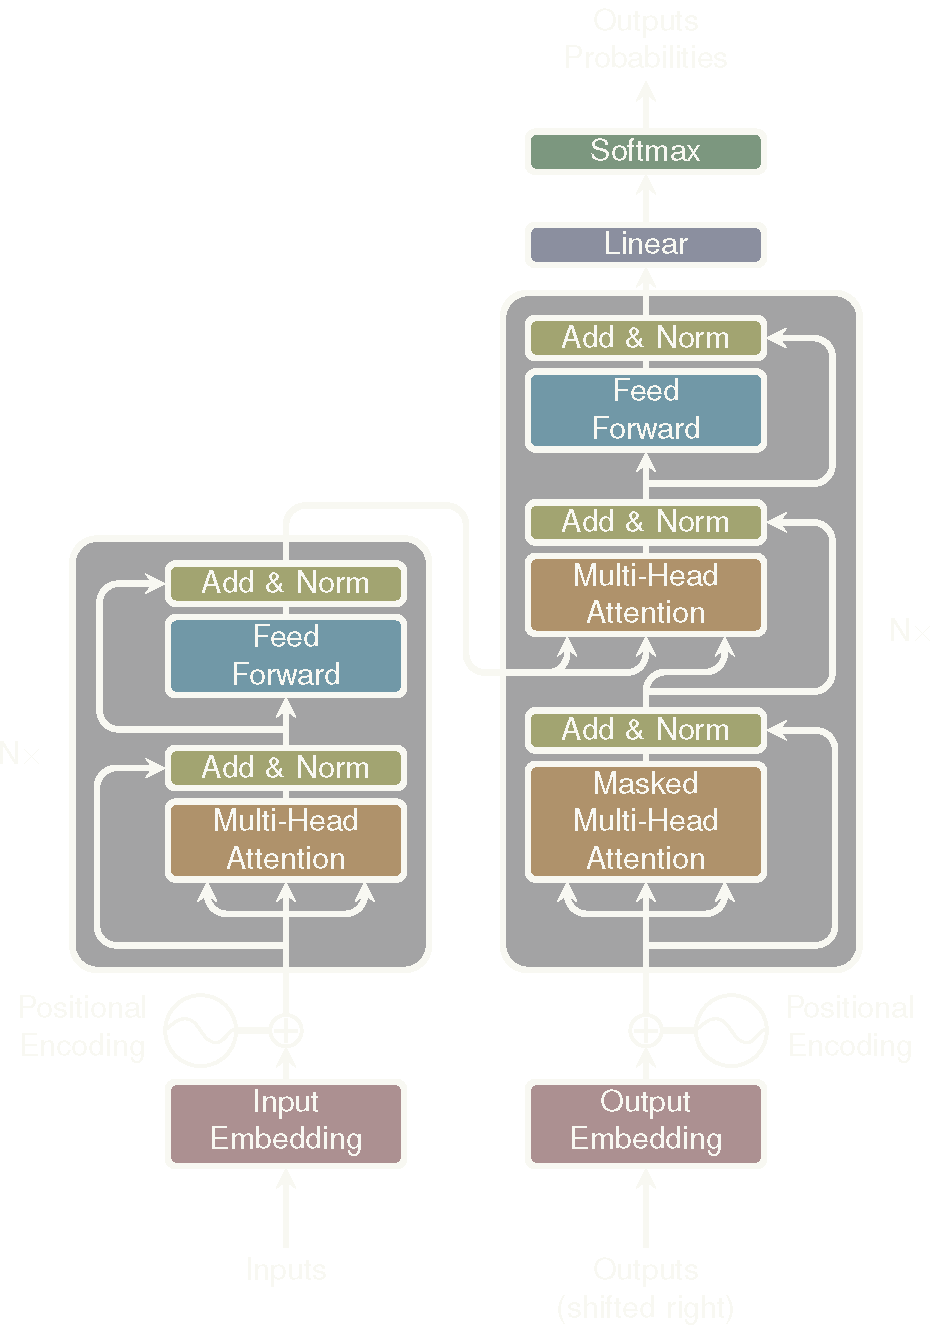
\includegraphics[width=0.6\textwidth]{images/ML_logo_v3.png}\\
            \caption{``The Transformer'' Recreated in TikZ from \href{https://proceedings.neurips.cc/paper_files/paper/2017/file/3f5ee243547dee91fbd053c1c4a845aa-Paper.pdf}{``Attention Is All You Need''}}
        \end{figure}

        % Horizontal line above the title in 'horange' color
        \textcolor{draculapink}{\rule{\textwidth}{1.0pt}}

        \vspace{2em}

        {\huge \textbf{\titlestandin}}

        \vspace{1em} % Space between the title and the bottom line

        \textcolor{draculapink}{\rule{\textwidth}{1.0pt}}

        \vspace*{1\baselineskip}

        {\LARGE \textbf{\cussubtitle}}

        \begin{large}
            \vspace*{2\baselineskip}

            \emph{Author} \\[1ex]
            %Submitted by \\[\baselineskip]
            {\Large Paul Beggs \\ \par} % Editor list
            {\href{mailto:PaulBeggs03@gmail.com}{{PaulBeggs03@gmail.com}}}\\ % Editor affiliation

        \end{large}
    \end{center}
\end{titlepage}
\pagebreak

\chapter*{Acknowledgements and Roadmap}

Thank you to \textit{Aurélien Géron} for writing the book \textit{Hands-On Machine Learning with Scikit-Learn, Keras, and TensorFlow}. This document is a compilation of notes taken while reading the book. The notes are not exhaustive and are meant to be a reference for myself. \\

Attribution: “\textit{Hands-On Machine Learning with Scikit-Learn, Keras, and TensorFlow} by Aurélien Géron. Copyright 2023 Aurélien Géron, 978-1-098-12597-4.” \\

This book is organized in two parts. Part I, “The Fundamentals of Machine Learning”, covers the following topics:
\begin{itemize}
    \item What machine learning is, what problems it tries to solve, and the main categories and fundamental concepts of its systems
    \item The steps in a typical machine learning project
    \item Learning by fitting a model to data
    \item Optimizing a cost function
    \item Handling, cleaning, and preparing data
    \item Selecting and engineering features
    \item Selecting a model and tuning hyperparameters using cross-validation
    \item The challenges of machine learning, in particular underfitting and overfitting (the bias/variance trade-off)
    \item The most common learning algorithms: linear and polynomial regression, logistic regression, k-nearest neighbors, support vector machines, decision trees, random forests, and ensemble methods
    \item Reducing the dimensionality of the training data to fight the “curse of dimensionality”
    \item Other unsupervised learning techniques, including clustering, density estimation, and anomaly detection
\end{itemize}
Part II, “Neural Networks and Deep Learning”, covers the following topics:
\begin{itemize}
    \item What neural nets are and what they’re good for
    \item Building and training neural nets using TensorFlow and Keras
    \item The most important neural net architectures: feedforward neural nets for tabular data, convolutional nets for computer vision, recurrent nets and long short-term memory (LSTM) nets for sequence processing, encoder–decoders and transformers for natural language processing (and more!), autoencoders, generative adversarial networks (GANs), and diffusion models for generative learning
    \item Techniques for training deep neural nets
    \item How to build an agent (e.g., a bot in a game) that can learn good strategies through trial and error, using reinforcement learning
    \item Loading and preprocessing large amounts of data efficiently
    \item Training and deploying TensorFlow models at scale
\end{itemize}
The first part is based mostly on Scikit-Learn, while the second part uses TensorFlow and Keras.


%-%-%-%-%-%-%-%-%-%-%-%-%-%-%-%-%-%-%-%-%-%-%-%-%-%-%-%-%-%-%-%-%-%-%-%-%-%-%

%%% Table of Contents %%%


% -%-%-%-%-%-%-%-%-%-%-%-%-%-%-%-%-%-%-%-%-%-%-%-%-%-%-%-%-%-%-%-%-%-%-%-%-%-%

% Helper command to fix header for double paged ToC.
% Temporarily adjust section marks for Table of Contents
\begin{spacing}{1} % Can change spacing between entries in TOC
    \renewcommand{\contentsname}{\Large\textbf{Table of Contents}} % Can rename here
    \markboth{}{} % Clear the header marks for TOC
    \pagestyle{fancy} % Ensure fancy style is active
    \fancyhead[R]{Table of Contents} % Set TOC-specific header manually
    \tableofcontents
    \addtocontents{toc}{\protect\enlargethispage{\baselineskip}}
\end{spacing}

% Reset the headers to default for the rest of the document
\fancyhead[R]{\leftmark}




% -%-%-%-%-%-%-%-%-%-%-%-%-%-%-%-%-%-%-%-%-%-%-%-%-%-%-%-%-%-%-%-%-%-%-%-%-%-%

\part{The Fundamentals of Machine Learning}

\chapter{The Machine Learning Landscape}
\vspace*{-0.25in}
\section{Introduction}
\label{sec:intro}

We will start by defining machine learning and why one would want to use it. Then, we will look at supervised versus unsupervised learning and their variants, online versus batch learning, and instance-based versus model-based learning. Then, we will look at the workflow of a typical ML project and discuss the main challenges and how to evaluate and fine-tune a machine learning system. \\

\cyanit{Machine Learning} is the science (and art) of programming computers, so they can \textit{learn} from data. \\

A more engineering based definition:
\begin{quote}
    \textit{A computer program is said to learn from experience $E$ with respect to some class of tasks $T$ and performance measure $P$, if its performance at tasks in $T$, as measured by $P$, improves with experience $E$.} \\
    \quoteAuthor{Tom Mitchell, 1997}
\end{quote}

\section{Why Use Machine Learning?}
\label{sec:why_use_ml}

Machine learning is good for the following main points:
\begin{itemize}
    \item Problems for which existing solutions require a lot of fine-tuning or long lists of rules (a machine learning model can often simplify code and perform better than the traditional approach)
    \item Complex problems for which using a traditional approach yields no good solution (the best machine learning techniques can perhaps find a solution)
    \item Fluctuating environments (a machine learning system can easily be retrained on new data, always keeping it up to date)
    \item Getting insights about complex problems and large amounts of data
\end{itemize}

\subsection{Application Examples}
\label{subsec:application_examples}

Machine learning is used in many applications, including:
\begin{nobullet}
\nobulletitem{Analyzing images of products on a production line to automatically classify them}
    \begin{nobullet}
        \item This is image classification, typically performed using convolutional neural networks (CNNs; see Chapter 14) or sometimes transformers (see Chapter 16).
    \end{nobullet}
\nobulletitem{Detecting tumors in brain scans}
    \begin{nobullet}
        \item This is semantic image segmentation, where each pixel in the image is classified (as we want to determine the exact location and shape of tumors), typically using CNNs or transformers.
    \end{nobullet}
\nobulletitem{Automatically classifying news articles}
    \begin{nobullet}
        \item This is natural language processing (NLP), and more specifically text classification, which can be tackled using recurrent neural networks (RNN), but transformers work even better (see Chapter 16).
    \end{nobullet}
\nobulletitem{Automatically flagging offensive comments on discussion forums}
    \begin{nobullet}
        \item This is also text classification, using the same NLP tools.
    \end{nobullet}
\nobulletitem{Summarizing long documents automatically}
    \begin{nobullet}
        \item This is a branch of NLP called text summarization, again using the same tools.
    \end{nobullet}
\nobulletitem{Creating a chatbot or personal assistant}
    \begin{nobullet}
        \item This involves many NLP components, including natural language understanding (NLU) and question-answering modules.
    \end{nobullet}
\nobulletitem{Forecasting your company's revenue next year, based on many performance metrics}
    \begin{nobullet}
        \item This is a regression task (i.e., predicting values) that may be tackled using any regression model, such as a linear regression or polynomial regression model (see Chapter 4), a regression support vector machine (see Chapter 5), a regression random forest (see Chapter 7), or an artificial neural network (see Chapter 10). If you want to take into account sequences of past performance metrics, you may want to use RNNs, CNNs, or transformers (see Chapters 15 and 16).
    \end{nobullet}
\nobulletitem{Marking your app react to voice commands}
    \begin{nobullet}
        \item This is speech recognition, which requires processing audio samples: since they are long and complex sequences, they are typically pocessed using RNNs, CNNs, or transformers (see Chapters 15 and 16).
    \end{nobullet}
\nobulletitem{Detecting credit card fraud}
    \begin{nobullet}
        \item This is anomaly detection, which can be tackled using isolation forests, Gaussian mixture models (see Chapter 9), or autoencoders (see Chapter 17).
    \end{nobullet}
\nobulletitem{Segmenting clients based on their purchases so that you can design a different marketing strategy for each segment}
    \begin{nobullet}
        \item This is clustering, which can be achieved using \textit{k}-means, DBSCAN, and more (see Chapter 9).
    \end{nobullet}
\nobulletitem{Recommending a product that a client may be interested in, based on past purchases}
    \begin{nobullet}
        \item This is a recommender system. One approach is to feed past purchases (and other information about the client) to an artificial neural network (see Chapter 10), and get it to output the most likely next purchase. This neural net would typically be trained on past sequences of purchases across all clients. 
    \end{nobullet}
\nobulletitem{Building an intelligent bot for a game}
    \begin{nobullet}
        \item This is often tackled using reinforcement learning (RL; see Chapter 18), which is a branch of machine learning that trains agents (Such as bots) to pick the actions that will maximize their rewards over time (e.g., a bot may get a reward every time the player loses some life points), within a given environment (such as the game). The famous AlphaGo program that beat the world champion at the game of Go was built using RL.
    \end{nobullet}
\end{nobullet}

\section{Types of Machine Learning Systems}
\label{sec:types_of_ml_systems}

Machine learning systems can be classified into several categories, depending on the type of data they are trained on and the type of tasks they are designed to perform. The main categories are:
\begin{itemize}
    \item How they are supervised during training (supervised, unsupervised, or semi-supervised, self-supervised, and others)
    \item Whether or not they can learn incrementally on the fly (online versus batch learning)
    \item Whether they work by simply comparing new data points to known data points, or instead by detecting patterns in the training data and building a predictive model, much like scientists do (instance-based versus model-based learning)
\end{itemize}

\subsection{Training Supervision}
\label{subsec:training_supervision}

This subsection goes over the main types of supervision used in machine learning: supervised, unsupervised, semi-supervised, self-supervised, and reinforcement learning. 

\subsubsection{Supervised Learning}
\label{subsubsec:supervised_learning}

\cyanit{Supervised Learning} is when you feed an algorithm a training set of labeled examples, and the algorithm learns to predict the labels for new instances. \\

\cyanit{Classification} a spam filter is a good example of this: it is trained with many example emails along with their \textit{class} (spam or ham), and it must learn how to classify new emails. \\

\cyanit{Regression} is when the labels are continuous values (e.g., predicting the price of a house). Training involves giving the model many examples of cars, including both their features and their targets (i.e., their prices).
\newpage
\begin{notebox}
    The words \textit{target} and \textit{label}  are often used interchangeably, but \textit{target} is more common in regression tasks, while \textit{label} is more common in classification tasks. Moreover, \textit{features} are sometimes called \textit{predictors} or \textit{attributes}. These terms may refer to individual samples (e.g., ``this car's mileage feature is equal to 15,000''), or to all samples (e.g., ``the mileage feature is strongly correlated with price.'').
\end{notebox}

\subsubsection{Unsupervised Learning}
\label{subsubsec:unsupervised_learning}

\cyanit{Unsupervised Learning} is when you only feed the algorithm a training set of unlabeled examples, and the algorithm tries to learn the structure of the data. \\

Consider the example of running a website that collects data from shoppers. You can run a \cyanit{clustering} algorithm on the data to group similar shoppers together. The algorithm will find connections between the shoppers without your assistance. For example, it might notice that 40\% of shoppers are teenagers who buy candy on weekdays after school, and 20\% are adults who only buy vegetables on the weekend. If you use \cyanit{hierarchical clustering} you can subdivide these groups into smaller groups, such as ``teenagers who buy candy on weekdays after school'' and ``teenagers who buy candy on weekends''. \\

\cyanit{Visualization} algorithms take complex, unlabeled data, and output a 2D or 3D representation that can easily be plotted. They preserve as much structure as possible (e.g., trying to keep separate clusters in the input space from overlapping in the visualization) so that you can perhaps identify unsuspected patterns. \\

A related task is \cyanit{dimensionality reduction}, in which the goal is to simplify the data without losing too much information. You could merge several correlated features into one. For example, you could combine the features ``height'' and ``weight'' into a single feature called ``body mass index (BMI)''. This is called \cyanit{feature extraction}.

\begin{tipbox}
    Reducing the number of dimensions in training data by utilizing these dimensionality reduction algorithms will make the later machine learning algorithm run much faster, take up less memory and disk space, and in some cases, improve the performance of the algorithm.
\end{tipbox}

\cyanit{Anomaly detection} is a special case of unsupervised learning, where the goal is to identify rare items, events, or observations that raise suspicions by differing significantly from the majority of the data. For example, you could use anomaly detection to identify fraudulent credit card transactions. \\

Similarly, \cyanit{novelty detection} is used to detect new instances that look different from all other instances in the training set. The caveat for using this method, is that your training set must be ``clean'' (i.e., devoid of any instance that you would like the algorithm to detect). For example, if you have thousands of images of different dogs and 1\% of these are Chihuahuas, then a novelty detection algorithm should not treat new pictures of Chihuahuas as novelties. On the other hand, anomaly detection algorithms may consider these dogs as so rare and different from other dogs that they would likely classify them as anomalies. \\

The final unsupervised task is \cyanit{association rule learning}, which is used to discover interesting relations between variables in large databases. For example, suppose you own a supermarket. Running an association rule on your sales logs may reveal that people who purchase barbecue sauce and potato chips also tend to buy steak. Thus, you may want to place these items close to each other in your store.

\subsubsection{Semi-Supervised Learning}
\label{subsubsec:semi_supervised_learning}

Since labeling is often time-consuming and costly, some algorithms can deal with data that's partially labeled. This is called \cyanit{semi-supervised learning}. \\

Google Photos uses semi-supervised learning to identify people in your photos. Once all your family photos are uploaded to the service, it automatically recognizes that the same person A shows up in photos 1, 5, and 11, while another person B shows up in photos 2, 5, and 7. This is the \textit{unsupervised} part of the algorithm that utilizes clustering. \\

Most semi-supervised learning algorithms are combinations of unsupervised and supervised learning algorithms. For example, a clustering algorithm may group similar instances together, and then every unlabeled instance can be labeled with the most common label in its cluster. Once the whole dataset is labeled, a supervised learning algorithm can be trained on it.

\subsubsection{Self-Supervised Learning}
\label{subsubsec:self_supervised_learning}





\setcounter{chapter}{1}





%-%-%-%-%-%-%-%-%-%-%-%-%-%-%-%-%-%-%-%-%-%-%-%-%-%-%-%-%-%-%-%-%-%-%-%-%-%-%
\end{document}
%-%-%-%-%-%-%-%-%-%-%-%-%-%-%-%-%-%-%-%-%-%-%-%-%-%-%-%-%-%-%-%-%-%-%-%-%-%-%

%-%-%-%-%-%-%-%-%-%-%-%-%-%-%-%-%-%-%-%-%-%-%-%-%-%-%-%-%-%-%-%-%-%-%-%-%-%-%